%        File: topology.tex
%     Created: Thu Nov 09 01:00 PM 2006 C
% Last Change: Thu Nov 09 01:00 PM 2006 C
%
% This file is part of Netsukuku
% (c) Copyright 2007 Andrea Lo Pumo aka AlpT <alpt@freaknet.org>
%
% This source code is free software; you can redistribute it and/or
% modify it under the terms of the GNU General Public License as published 
% by the Free Software Foundation; either version 2 of the License,
% or (at your option) any later version.
%
% This source code is distributed in the hope that it will be useful,
% but WITHOUT ANY WARRANTY; without even the implied warranty of
% MERCHANTABILITY or FITNESS FOR A PARTICULAR PURPOSE.
% Please refer to the GNU Public License for more details.
%
% You should have received a copy of the GNU Public License along with
% this source code; if not, write to:
% Free Software Foundation, Inc., 675 Mass Ave, Cambridge, MA 02139, USA.
%

\documentclass[a4paper]{article}
\usepackage{color,graphicx}
\usepackage{amsmath}
\usepackage{amsthm}
\usepackage{amssymb}
\usepackage{amsfonts}
\RequirePackage{ifpdf} % running on pdfTeX?
\ifpdf
\usepackage[pdftex,bookmarks=true,
		   bookmarksnumbered=false,
		   bookmarksopen=false,
		   colorlinks=true,
		   linkcolor=webred] {hyperref}
\definecolor{webgreen}{rgb}{0, 0.5, 0} % less intense green
\definecolor{webblue}{rgb}{0, 0, 0.5} % less intense blue
\definecolor{webred}{rgb}{0.5, 0, 0}   % less intense red
\else
\newcommand{\href}[2]{ #1 }
\fi

%%%% Misc
\newcommand{\T}[1]{\textrm{#1}}
\newcommand{\see}[1]{\T{[\ref{#1},pg.\pageref{#1}]}}
\newcommand{\vedi}[1]{\T{vedi \see{#1}}}
\newcommand{\pgra}[1]{\left\{#1\right\}}
\newcommand{\pqua}[1]{\left[#1\right]}
\newcommand{\pton}[1]{\left(#1\right)}
\newcommand{\pass}[1]{\Big|#1\Big|}
\newcommand{\sist}[1]{{ \begin{cases} #1 \end{cases} }}
\newcommand{\eal}[1]{{\begin{align*} #1 \end{align*}}}
\def\ove#1{{\overline{#1}}}
\newcommand{\qq}{\qquad}
%% Defs
\def\*{{\times}}
\def\|{{\;\lor\;}}
\def\&{{\;\land\;}}
\def\-{{\setminus}}
\def\0{{\emptyset}}
\def\8{{\infty}}
\def\v{{\cup}}
\def\^{{\cap}}
\def\<{{\;\Leftarrow\;}}
\def\>{{\;\Rightarrow\;}}
\def\={{\;\Leftrightarrow\;}}
\def\({{\subseteq}}
\def\){{\supseteq}}
\def\'{{\;\;\;}}
\def\,{{,\;}}




\title{Netsukuku topology}
\author{http://netsukuku.freaknet.org\\AlpT (@freaknet.org)}
\begin{document}
\maketitle
\begin{abstract}
	In this document, we describe the fractal structure of the Netsukuku
	topology. Moreover, we show how it is possible to use the QSPN v2 on
	the high levels of the fractal.
\end{abstract}
\pagenumbering{roman}
\pagebreak
\begin{small}
  This document is part of Netsukuku.\\
  Copyright \copyright 2007 Andrea Lo Pumo aka AlpT $<$alpt@freaknet.org$>$.
  All rights reserved.

  This document is free; you can redistribute it and/or modify it
  under the terms of the GNU General Public License as published by
  the Free Software Foundation; either version 2 of the License, or
  (at your option) any later version.

  This document is distributed in the hope that it will be useful, but
  WITHOUT ANY WARRANTY; without even the implied warranty of
  MERCHANTABILITY or FITNESS FOR A PARTICULAR PURPOSE\@.  See the GNU
  General Public License for more details.

  You should have received a copy of the GNU General Public License
  along with this document; if not, write to the Free Software
  Foundation, Inc., 675 Mass Ave, Cambridge, MA 02139, USA.
\end{small}

\clearpage
\tableofcontents
\clearpage
\pagenumbering{arabic}


\section{Preface}
\label{sec:preface}

We're assuming that you already know the basics of the QSPN. If not, read the
QSPN document first: \cite{qspndoc}.

\section{The general idea}
\label{sec:general_idea}

The aim of Netsukuku is to be a (physical) scalable mesh network, completely
distributed and decentralised, anonymous and autonomous.

The software, which must be executed by every node of the net, has to be
unobtrusive. It has to use very few CPU and memory resources, in this way it
will be possible to run it inside low-performance computers, like Access Points,
embedded devices and old computers.

If this requirements are met, Netsukuku can be easily used to build a worldwide
distributed, anonymous and not controlled network, separated from the
Internet, without the support of any servers, ISPs or control authorities.

\section{Basic definitions}

\begin{description}
	\item[Node] We call \emph{node} any computer that is hooked up to the
		Netsukuku network.
	\item[Rnode] stands for \emph{in-Range Node}: given a node X, it is any other
		node directly linked to X, i.e. it's a neighbour of X.
	\item[Map] A map is a file, kept by each node, which contains all the
		necessary information about the network, f.e. routes and nodes
		status.
	\item[REM] stands route \emph{Route Efficiency Measure}. It is 
		a value that indicates the quality of a route. 
		REM can be calculated in various ways, f.e. by taking in
		account the total rtt and the bw capacity of the route.  We denote the REM of
a route $r$ as $REM(r)$.

\end{description}
Example:\\
\begin{figure}[h]
	\begin{center}
		\includegraphics[scale=0.5]{fig/segABC}
	\end{center}
	\caption{The nodes A,B and C}
\end{figure}
A is the rnode of B.\\
B is the rnode of A and C.\\
C is the rnode of B.

\section{Network topology}
\label{sec:net_topology}

A simple topology, which doesn't impose any structure on the network, can be
memorised with a simple map. In this map, all the information regarding the
nodes of the network have to be memorised. Surely, this kind of map cannot be
utilised by Netsukuku, because it would require too much memory.
For example, even if we store just one route to reach one node and even if
this route costs one byte, we would need 1Gb of memory for a network composed
by $10^9$ nodes (the current Internet).

For this reason, it's necessary to structure the network in a convenient
topology.

\subsection{Fractal topology}
\label{sec:fractal_topology}
\subsubsection{Level 1}
First of all we'll subdivide the network in groups of 256 nodes and we'll use
the following definitions:
\begin{description}
	\item[Gnode] means group node. It is a group of nodes, i.e. a set of
		nodes. Each node of the network belongs to just one gnode.\\
		A gnode contains a maximum of 256 nodes.\\
		By writing $n \in G$ we mean that the node $n$ belongs to the
		gnode $G$.
	\item[Bnode] stands for border node. It is a node which belongs to a
		gnode G, but that is also directly linked to at least one node
		of another gnode, i.e. some of its rnodes belongs to different
		gnodes than its.\\
		By writing $b \in G$ we mean that the bnode $b$ belongs to the
		gnode $G$.
\end{description}

Example:\\
\begin{figure}[h]
	\begin{center}
		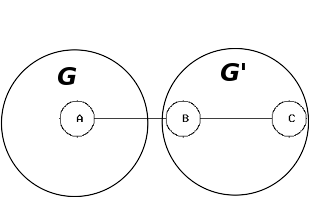
\includegraphics[scale=0.5]{fig/bnode}
	\end{center}
	\caption{The bnode A and B, belonging respectively to the gnode G and
	$G'$}
\end{figure}
$A \in G $, A is a node belonging to the gnode G, its rnode is B.\\
$B \in G'$, B is a node belonging to the gnode $G'$, its rnode is A.\\
A is a bnode of G, while B is a bnode of $G'$.

\subsubsection{Level n}
We further subdivide the network topology in \emph{groups of 256 groups of nodes}
and we continue to name them as gnode.\\
At this point, we repeat recursively this subdivision process until
we can group all the nodes of the network into a single gnode.

Doing so, we've structured the network in $n+1$ levels (from $0$ to $n$).\\
In the base level (level 0), there are 256 single nodes.\\
In the first level (level 1), there are 256 normal gnodes. Each of them
contains 256 single nodes.\\
In the second (level 2), 256 gnodes of level 1 forms a single \emph{group of
groups of nodes}.\\
In the third (level 3), there are 256 groups of 256 groups of 256 groups of
256 nodes.\\
Continuing in this way, we arrive at the last level (level $n$), where there
is a single group which contains the whole network.\\

The QSPN algorithm is able to operate independently on any level,
considering each gnode as a single node of level 0.
For this reason, we can view the Netsukuku topology as a fractal, where each
level is composed by single nodes.

\subsubsection*{Example}

Figure \ref{fig:fract_circle}\footnote{this figure has been taken from:
\href{http://www.ian.org/FX/Plugins.html}{http://www.ian.org/FX/Plugins.html}}
is an example of the fractal topology of Netsukuku.

\begin{figure}[h]
	\begin{center}
		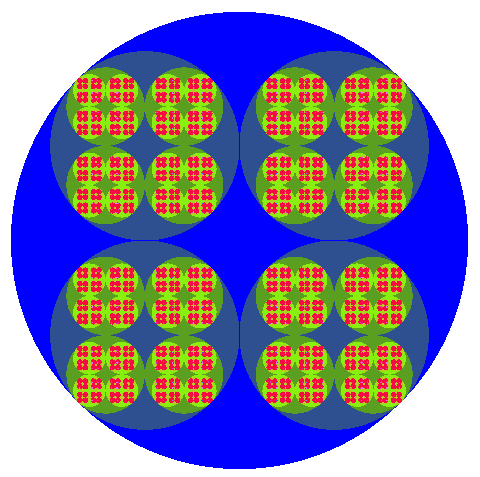
\includegraphics[scale=0.5]{fig/fractal_circle}
	\end{center}
	\caption{An example of the netsukuku topology structure}
	\label{fig:fract_circle}
\end{figure}

In this topology, each gnode contains four nodes, i.e. each group contains
four elements. The network is structured in 6 levels.\\
The red elements, are single nodes (level 0).\\
Four nodes forms a single group of nodes (level 1).\\
A single bright green circle is a 
				  group of groups of nodes (level 2).\\
The dark green circles are        groups of groups of groups of nodes (level 3).\\
The dark blue circle are          groups of groups of groups of groups of
nodes (level 4). \\
Finally, the bright blue circle is the gnode which contains the whole network
(level 5).

\subsubsection{Membership}
Let's assign a numeric ID to each (g)gnode, starting from the last level:
\begin{enumerate}
	\item in the last level ($n$) there's only one giant gnode, thus we assign
		to it the ID ``0''. Our global ID will be:
		\[
		0
		\]
	\item in $n-1$ there are 256 gnodes, which belongs to the gnode 0 of
		level $n$, thus we assign them the IDs from $0$ to $255$.
		The global ID becomes:
		\[
		0\cdot i\quad 0\le  i\le 255
		\]
	\item we repeat the step 2 recursively gaining an ID of this form:
		\[
		0\cdot i_{n-1}\cdot i_{n-2}\cdot \dots \cdot i_0 \quad 0\le i_j\le 255,\;0\le j\le n-1
		\]
	\item since the last level is always $0$, we'll omit it and we'll
		consider only the first $n$ levels.
\end{enumerate}
In a network with a maximum of $2^{32}$ nodes (the maximum allowed by the ipv4),
there would be five levels ($n=4$), where each gnode will be composed by 256 nodes.
Therefore, the ID will be in the usual IP form:
\[
0\dots255\cdot 0\dots255\cdot 0\dots255\cdot 0\dots255
\]
For example, a single node of level 0 of the network is:
\[
3\cdot 41\cdot 5\cdot 12
\]
That said, each gnode of the network belongs to only one combination of gnodes
of the various levels. In our previous example we have:
\begin{align*}
	&g_3=3\\
	&g_2=41\\
	&g_1=5\\
	&g_0=12
\end{align*}
where each $g_i$ corresponds to the gnode ID of the level $i$. Note that $g_0$
is the ID attributed to the single node, at level 0.

\subsection{Fractal map}
The advantages of using a fractal topology are clear.\\
The node $N$, instead of memorising information about each node of the whole
network, will keep only that regarding the gnodes where it belongs to.
Suppose the node $N$ had this ID:
\[
g_3\cdot g_2\cdot g_1\cdot g_0
\]
It will store in memory information regarding:
\begin{enumerate}
	\item the 256 single nodes which belongs to its same gnode of level 1,
		or in other words, the 256 nodes of the gnode $g_1$,
	\item the 256 gnodes gnodes which belongs to its same gnode of level
		2, of in other words, the 256 gnodes of the gnode $g_2$,
	\item finally, the 256 gnodes which belongs to the gnode $g_3$.
\end{enumerate}
Note that doing so, the node $N$ will be blind to all the other gnodes. For
example, it won't know any information regarding the single nodes which belong
to all the other gnodes of level 1 different from $g_1$.\\

Even with this lack of knowledge, as we'll see later, the node $N$ is still
able to reach all the other nodes of the network.
In conclusion, $N$ only needs $256n$ entries in its map, instead of $2^{32}$. 
To clarify the ideas suppose that each entry costs one byte. In the plain
topology we needed $4Gb$, while in the fractal one we just need $256\cdot 4\;
b= 1Kb$.

\subsubsection{IP v4 and v6}
Netsukuku is both compatible with ipv4 and ipv6.\\

In ipv4 there are a maximum of $2^{32}$ IPs, thus we have five levels $n=4$.\\
In ipv6 there are a maximum of $2^{128}$ IPs, thus $n=16$.

\subsubsection{Internal and external map}
For simplicity we divide the map of the node $N$, in the \emph{internal map} and in
the \emph{external} one.  The internal map contains information regarding the
nodes belonging to $g_1$. The external map describes all the other levels of
the topology.

\subsection{CIDR routing}
The QSPN, for each level, will build the routes necessary to connect each
(g)node to all the other (g)nodes of the same level. The routes will be saved
in the maps of each node.\\

If the node $N=g_3\cdot g_2\cdot g_1 \cdot g_0$ wants to reach a node $M$ which
belongs to different gnodes, f.e. $M=g_3\cdot g_2\cdot h_1 \cdot h_0$, it will
add a CIDR\cite{CIDR} route in the routing table of the kernel:\\
\emph{all the packets whose destination is $g_3\cdot g_2\cdot h_1 \cdot 0\dots
255$ will be forwarded to the gateway $X$}.\\

We'll see later how the gateway $X$ is chosen.

\section{The internal map and its myopia}
\label{sec:intmyopia}
We define a route $r_N$ of the node $N$ as the following tern:
\eal{&r_N:=(dst, gw, rem)\\
&\T{where }\\
&\qq \T{$dst$ is a node: the destination node of the route}\\
&\qq \T{$gw$ is a node: the gateway of the route}\\
&\qq \T{$rem$ is a number: the REM value of the route}
}
We'll use $ dst(r), gw(r), rem(r)$, to indicate respectively the first, second
and third element of the tern $r$.\\
Let $\textbf{R}$ be the set
of all routes of the node $N$ (note \footnote{for semplicity we are considering just one metric for all
the routes. However, it's easy to see that the following
propositions are valid for different metrics (just use a different set
$\textbf{R}_m$ for each metric $m$)}). We can define the following equivalence relation:
\eal{&\forall r,s\in \textbf{R}\;\;\;r\sim s \= dst(r)=dst(s) }
With $\ove r$ we indicate the equivalence class of $r$.\\
Consider the following subset of $\textbf{R}$:
\eal{&R=\pgra{r \in \textbf{R}\;|\;dst(r) \in G}\\
&\T{where $G$ is the gnode of level 1 such that $N\in G$}
}
At this point we can define the internal map of $N$ as the subset $M\( R$, such that
\eal{& \forall r\in M\;\;\forall s,t\in \ove r\;\T{with}\;s\neq t\;\;\; gw(s)\neq gw(t)
}
This means that when the node $N$ wants to save in $M$ a route $s$, which has
the same destination of a route $r\in M$, the following algorithm will be
adopted:
\eal{&\textbf{if}\' \exists t\in \ove r:\;gw(t)=gw(s)\\
&\qq \textbf{if}\' rem(t) < rem(s)\'\T{[s is better than t]}\\
&\qq\qq \T{overwrite t with s;}\\
&\qq \textbf{else}\' \T{do nothing};\\
&\textbf{else}\' \T{save s in $M$;}
}
The reason for the above definitions is that a node $N$, in order 
to reach any other node of the network will just need to know to which of its
neighbours send the packets.\\
A route saved in the internal map it's just a tern, not an ordinate sequence
of nodes, therefore the node $N$ doesn't know its entire path. For this
reason, we can say that the vision of the node $N$ of the entire net is myope,
or local. As we'll see later, this local vision can be easily applied to
higher levels. Note also that the QSPN v2 is indipendent from the above
definitions, i.e. it's way of working doesn't change.


\section{Flat levels}
\label{sec:flat}
From the point of view of the QSPN v2, the levels are ``flattened'', because
the propagation of an ETP or a CTP \footnote{for more info on the ETP and CTP,
see the QSPN document \cite{qspndoc}} inside the whole network is exactly as
before, briefly: a packet is propagated until it is interesting, the
subdvisions of nodes in gnodes are simply ignored . The only
added rule serves to economize space: 

let $T$ be a generic tracer packet and let $\pgra{a_i\;|\;i=1,2,\dots,n}$ be its finite sequence of nodes.
Every subsequence \[\pgra{a_h\in G\;|\;h=i+1,i+2,\dots,j-1}\]
such that $a_i,a_j\notin G$, where $G$ is a gnode of any level, is replaced by
the ID of $G$. The rem associated with the ID of $G$ is the summation of the
rem of every term of the subsequence.\\
This rule is valid for any level, it is called the \emph{group rule}.\\
Some examples:
\begin{enumerate}
	\item The tracer packet
		\eal{&11.22.1,\;11.22.80,\;11.22.35}
		cannot be grouped, because $a_i\in 11.22\;\forall i =1,2,3$
	\item The tracer packet
		\eal{&11.22.1,\;11.22.80,\;11.22.35,\;11.44.13}
		can be grouped in the following tracer packet:
		\eal{&11.22.*,\;11.44.13}
	\item The tracer packet
		\eal{&11.22.1,\;11.22.80,\;11.22.35,\;11.44.13,\;55.32.20}
		can be grouped in the following tracer packet:
		\eal{&11.*,\;55.32.30\'\'(1)}
\end{enumerate}
The description of a route in the external map is local, as in the internal
map (see \ref{sec:intmyopia}). For example, when the node $55.32.12$ receives
the tracer packet $(1)$, it will save the following route:
\eal{&(dst=11.*=\T{any node of the gnode $11$},\;gw=\T{my neighbour
$55.32.20$},\;rem)
}
Finally, the set $M$ used for the description of the ETP in the QSPN document
\cite{qspndoc}, is changed from the set of all routes of the internal map to
the set of all routes (internal and external).

\section{Network dynamics}
When a part of the network changes considerably, the maps of the involved
levels must be updated.

\subsection{Radar}
Every node has its own radar, which periodically sends a broadcast request to
all its (physical) near nodes. By collecting the replies, the radar is able to
determine the active rnodes of the node and the quality of its links.

\subsection{Level 0}
\label{sec:netdyn-level0}
In level 0, a CTP is sent every time a node joins the network, dies or every
time the change of the quality of a link exceeds a predefined delta value. The
CTP is also is restricted to the gnode where it has been originated: a
bnode won't send it to external nodes.\\
\newline
When a node joins, it won't send a CTP, only its rnodes will.
Their CTP will be directed to the node. More formally:\\
if the node $n$ joins, that is if the node $n$ creates a link
with the nodes $r_1,\dots,r_n$, with $n\ge 1$, then a CTP will
be sent by each rnode $r_i$ \emph{only} to $n$. This means that if $r_j$ is connected to a node $s$, when
$n$ joins, $r_j$ will send the CTP only to $n$ and not to
$s$.\\
This saves the propagation of two CTP in the following situation:
\[\dots \leftrightarrow A\leftrightarrow B\leftrightarrow C\leftrightarrow\dots\]
suppose that the node $B$ joins. As a consequence of the rule we've described,
the node $C$ will send a CTP to $B$ and $A$ to $B$, thus only two distinct CTP are
generated. Their path is $A\rightarrow B\rightarrow C\rightarrow \dots$ and
the reverse. If instead the node $B$ sends a CTP to $C$ and then $A$ to $B$,
two distinct CTP will explore the same verse: $B\rightarrow
C\rightarrow\dots $ and $A\rightarrow B\rightarrow C\rightarrow \dots$, the
same is for the reverse, thus, in total, four distinct CTP are propagated.\\
\newline
Let $A\stackrel{l}{\leftrightarrow}B$ be a link. If its quality changes $B$
will send a CTP to $A$ and vice-versa.\\
\newline
When a node dies, all its rnodes will send a CTP to all their rnodes. The CTP
will include, as the first hop, the ID of the dead node, with a flag which
indicates its death. For example:
\[A\leftrightarrow B\leftrightarrow C\leftrightarrow\dots\]
if $A$ dies, then $B$ will send the following CTP to $C$:
$\stackrel{+}{A}\;\rightarrow B$\\
\newline
In order to prevent false positives, the nodes won't immediately send the CTP, but
will wait a small amount of time. Only if the change persists, they will send it.

\subsection{Hooking phase}
A new node joins the network when it has been able to create at least one
physical link to an active Netsukuku node and when it has correctly executed
the hooking procedure. In this paragraph, we describe loosely the hooking
phase of a new node.

Suppose that the node $n$ has established a physical link to at least one Netsukuku
node. In order to become an active Netsukuku node, $n$ has to \emph{hook} to
its rnodes.

During the hook, $n$ will exchange vital information with its rnodes,
it will choose its new IP and it will finally become part of a gnode.

The hook procedure is formed by these general steps:
\begin{enumerate}
	\item The node $n$ chooses an IP in the range of $10.0.0.1 \le IP \le
		10.0.0.255$.
	\item It launches the first radar to see what its rnodes are. If not a
		single node is found, it creates a new gnode and ends hooking
		phase.
	\item At this point, $n$ asks to its nearer rnode the list of all the
		available free nodes presents inside the gnode of the rnode.\\
		If the rnode rejects the request (the gnode might be full),
		the node $n$ contacts another rnode.
	\item $n$ chooses an IP from the received list of free nodes and sets
		it on its network interface.
	\item $n$ will then download the external map from the same rnode.
		Looking at the external map, it will be able to determine if
		it has to create a new gnode. If it has, it creates it and
		ends the hooking.
	\item $n$ gets the internal and the bnode map from the same rnode.
	\item $n$ launches a second radar and updates its routing table.
	\item All the rnodes of $n$ send a CTP to update the maps.
\end{enumerate}


\subsection{Gnode hook}
When a node creates a new gnode, it will choose a random gnode ID, and thus
a random ip.\\
Suppose that two isolated gnodes get the same gnode ID. When they will be
linked, they'll enter in conflict.\\
The solution to this problem is to let each new gnode hook as a normal node
would. You can find more information about this in the NTK\_RFC 001\cite{gnodecontiguity}.

\section{ChangeLog}
\begin{itemize}
	\item \verb|July 2007|
		\begin{enumerate}
			\item Internal and external map structure redisigned:
				(see \ref{sec:intmyopia})
			\item The bnode map is no more necessary.
			\item Flat levels simplified.
		\end{enumerate}
	\item \verb|March 2007|
		\begin{itemize}
			\item Description of the Flat levels (sec. \ref{sec:flat})
			\item Section \ref{sec:netdyn-level0} ``Network dynamics - Level 0'' expanded.
			\item Section ``Network
				dynamics - Level n'' updated: the references to
				the pre-Flatlevels REM metric have been
				removed.
		\end{itemize}
	\item \verb|October 2006|\\
		Initial release.
\end{itemize}

%%%%%%%%%%%%%%%%
% Bibliography %
%%%%%%%%%%%%%%%%
\begin{thebibliography}{99}
	\bibitem{qspndoc} QSPN document:
		\href{http://netsukuku.freaknet.org/doc/main\_doc/qspn.pdf}{qspn.pdf}
	\bibitem{ntksite} Netsukuku website:
		\href{http://netsukuku.freaknet.org/}{http://netsukuku.freaknet.org/}
	\bibitem{CIDR} CIDR routing:
		\href{http://en.wikipedia.org/wiki/Classless\_Inter-Domain\_Routing}{Classless\_Inter-Domain\_Routing in Wikipedia}
	\bibitem{gnodecontiguity} NTK\_RFC 001:
		\href{http://lab.dyne.org/Ntk\_gnodes\_contiguity}{Gnode contiguity}
\end{thebibliography}
\newpage

\begin{center}
\verb|^_^|
\end{center}
\end{document}
